\documentclass[french]{article}
\usepackage[T1]{fontenc}
\usepackage{fullpage}
\usepackage{babel}
\usepackage{hyperref}
\usepackage{graphicx}
\usepackage[justification=centering]{caption}
\usepackage{amsmath}
\usepackage{amssymb}
\usepackage{listings}
\usepackage{xcolor}
\usepackage{parskip}

\lstset{
    inputencoding = utf8,  % Input encoding
    extendedchars = true,  % Extended ASCII
    literate      =        % Support additional characters
      {á}{{\'a}}1  {é}{{\'e}}1  {í}{{\'i}}1 {ó}{{\'o}}1  {ú}{{\'u}}1
      {Á}{{\'A}}1  {É}{{\'E}}1  {Í}{{\'I}}1 {Ó}{{\'O}}1  {Ú}{{\'U}}1
      {à}{{\`a}}1  {è}{{\`e}}1  {ì}{{\`i}}1 {ò}{{\`o}}1  {ù}{{\`u}}1
      {À}{{\`A}}1  {È}{{\`E}}1  {Ì}{{\`I}}1 {Ò}{{\`O}}1  {Ù}{{\`U}}1
      {ä}{{\"a}}1  {ë}{{\"e}}1  {ï}{{\"i}}1 {ö}{{\"o}}1  {ü}{{\"u}}1
      {Ä}{{\"A}}1  {Ë}{{\"E}}1  {Ï}{{\"I}}1 {Ö}{{\"O}}1  {Ü}{{\"U}}1
      {â}{{\^a}}1  {ê}{{\^e}}1  {î}{{\^i}}1 {ô}{{\^o}}1  {û}{{\^u}}1
      {Â}{{\^A}}1  {Ê}{{\^E}}1  {Î}{{\^I}}1 {Ô}{{\^O}}1  {Û}{{\^U}}1
      {œ}{{\oe}}1  {Œ}{{\OE}}1  {æ}{{\ae}}1 {Æ}{{\AE}}1  {ß}{{\ss}}1
      {ẞ}{{\SS}}1  {ç}{{\c{c}}}1 {Ç}{{\c{C}}}1 {ø}{{\o}}1  {Ø}{{\O}}1
      {å}{{\aa}}1  {Å}{{\AA}}1  {ã}{{\~a}}1  {õ}{{\~o}}1 {Ã}{{\~A}}1
      {Õ}{{\~O}}1  {ñ}{{\~n}}1  {Ñ}{{\~N}}1  {¿}{{?`}}1  {¡}{{!`}}1
      {°}{{\textdegree}}1 {º}{{\textordmasculine}}1 {ª}{{\textordfeminine}}1
      {£}{{\pounds}}1  {©}{{\copyright}}1  {®}{{\textregistered}}1
      {«}{{\guillemotleft}}1  {»}{{\guillemotright}}1  {Ð}{{\DH}}1  {ð}{{\dh}}1
      {Ý}{{\'Y}}1    {ý}{{\'y}}1    {Þ}{{\TH}}1    {þ}{{\th}}1    {Ă}{{\u{A}}}1
      {ă}{{\u{a}}}1  {Ą}{{\k{A}}}1  {ą}{{\k{a}}}1  {Ć}{{\'C}}1    {ć}{{\'c}}1
      {Č}{{\v{C}}}1  {č}{{\v{c}}}1  {Ď}{{\v{D}}}1  {ď}{{\v{d}}}1  {Đ}{{\DJ}}1
      {đ}{{\dj}}1    {Ė}{{\.{E}}}1  {ė}{{\.{e}}}1  {Ę}{{\k{E}}}1  {ę}{{\k{e}}}1
      {Ě}{{\v{E}}}1  {ě}{{\v{e}}}1  {Ğ}{{\u{G}}}1  {ğ}{{\u{g}}}1  {Ĩ}{{\~I}}1
      {ĩ}{{\~\i}}1   {Į}{{\k{I}}}1  {į}{{\k{i}}}1  {İ}{{\.{I}}}1  {ı}{{\i}}1
      {Ĺ}{{\'L}}1    {ĺ}{{\'l}}1    {Ľ}{{\v{L}}}1  {ľ}{{\v{l}}}1  {Ł}{{\L{}}}1
      {ł}{{\l{}}}1   {Ń}{{\'N}}1    {ń}{{\'n}}1    {Ň}{{\v{N}}}1  {ň}{{\v{n}}}1
      {Ő}{{\H{O}}}1  {ő}{{\H{o}}}1  {Ŕ}{{\'{R}}}1  {ŕ}{{\'{r}}}1  {Ř}{{\v{R}}}1
      {ř}{{\v{r}}}1  {Ś}{{\'S}}1    {ś}{{\'s}}1    {Ş}{{\c{S}}}1  {ş}{{\c{s}}}1
      {Š}{{\v{S}}}1  {š}{{\v{s}}}1  {Ť}{{\v{T}}}1  {ť}{{\v{t}}}1  {Ũ}{{\~U}}1
      {ũ}{{\~u}}1    {Ū}{{\={U}}}1  {ū}{{\={u}}}1  {Ů}{{\r{U}}}1  {ů}{{\r{u}}}1
      {Ű}{{\H{U}}}1  {ű}{{\H{u}}}1  {Ų}{{\k{U}}}1  {ų}{{\k{u}}}1  {Ź}{{\'Z}}1
      {ź}{{\'z}}1    {Ż}{{\.Z}}1    {ż}{{\.z}}1    {Ž}{{\v{Z}}}1
      % ¿ and ¡ are not correctly displayed if inconsolata font is used
      % together with the lstlisting environment. Consider typing code in
      % external files and using \lstinputlisting to display them instead.      
  }



\definecolor{codegreen}{rgb}{0,0.6,0}
\definecolor{codegray}{rgb}{0.5,0.5,0.5}
\definecolor{codepurple}{rgb}{0.58,0,0.82}
\definecolor{backcolour}{rgb}{0.95,0.95,0.92}

\lstdefinestyle{mystyle}{
    backgroundcolor=\color{backcolour},   
    commentstyle=\color{codegreen},
    keywordstyle=\color{magenta},
    numberstyle=\tiny\color{codegray},
    stringstyle=\color{codepurple},
    basicstyle=\ttfamily\footnotesize,
    breakatwhitespace=false,         
    breaklines=true,                 
    captionpos=b,                    
    keepspaces=true,                 
    numbers=left,                    
    numbersep=5pt,                  
    showspaces=false,                
    showstringspaces=false,
    showtabs=false,                  
    tabsize=2
}

\lstset{style=mystyle}
\setlength{\parindent}{0pt}

\hypersetup{
  colorlinks=true,
  linkcolor=black,
  urlcolor=blue
}

\graphicspath{ {./img/} }
\title{%
    \huge IArgus  \\
    \bigskip
    \large E3 - Mise en situation \\ 
    Développeur en Intelligence Artificielle,
    titre professionnel enregistré au RNCP - École IA Microsoft by Simplon
    \vfill
    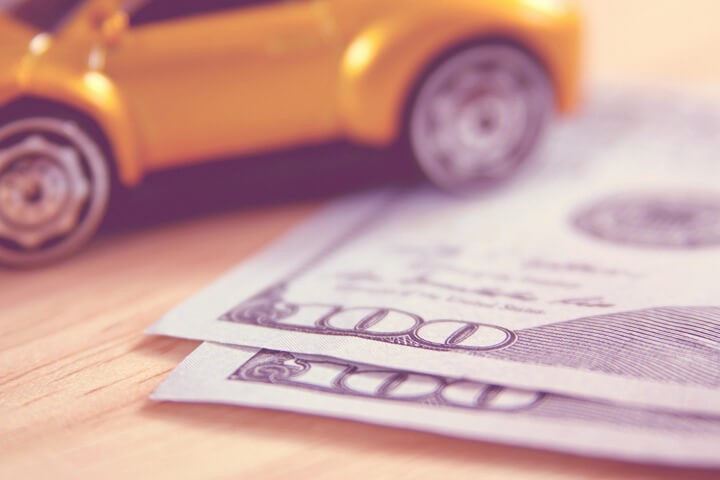
\includegraphics[width=14cm]{selling-your-old-car.jpg}
    \vfill}
\date{23 mars 2024}
\author{par Vincent Papelard}

\begin{document}
    \renewcommand{\contentsname}{Table des Matières}
    \renewcommand{\refname}{Références}
    \maketitle
    \pagenumbering{arabic}
    \pagenumbering{gobble}
    \newpage
    \tableofcontents
    \newpage
    \pagenumbering{arabic}

    \section*{Introduction}
    Depuis bientôt un siècle, l'Argus est le magazine de référence pour estimer la valeur d'un véhicule d'occasion. Fort de son statut en France, l'hebdomadaire a décidé de s'attaquer au marché américain en lançant son nouveau service, IArgus, aux États-Unis. Ce service en ligne proposera une IA qui estimera automatiquement le juste prix d'un véhicule en se basant sur des caractéristiques comme son modèle, son année de vente, son kilométrage...
    La direction de l'Argus a fait appel à nous pour développer ce nouveau service et leur livrer avec toute la documentation nécessaire à sa mise en place, puis intégrer ce modèle à l'application IArgus qu'ils ont créée.

    La totalité du code relatif à ce dossier est disponible sur \href{https://github.com/vinpap/iargus}{GitHub}.
    \section{Contexte}
    \subsection{L'application de départ}
    Dans l'optique d'accueillir ce nouveau service, les développeurs web embauchés par l'Argus ont créé un site web qui comporte un formulaire permettant aux utilisateurs d'entrer les caractéristiques d'une voiture. C'est là que nous intervenons : nos clients de l'Argus souhaitent que la validation de ce formulaire envoie une requête à une intelligence artificielle qui estimera le meilleur prix de vente pour la voiture de l'utilisateur.
    \begin{figure}[h!]
        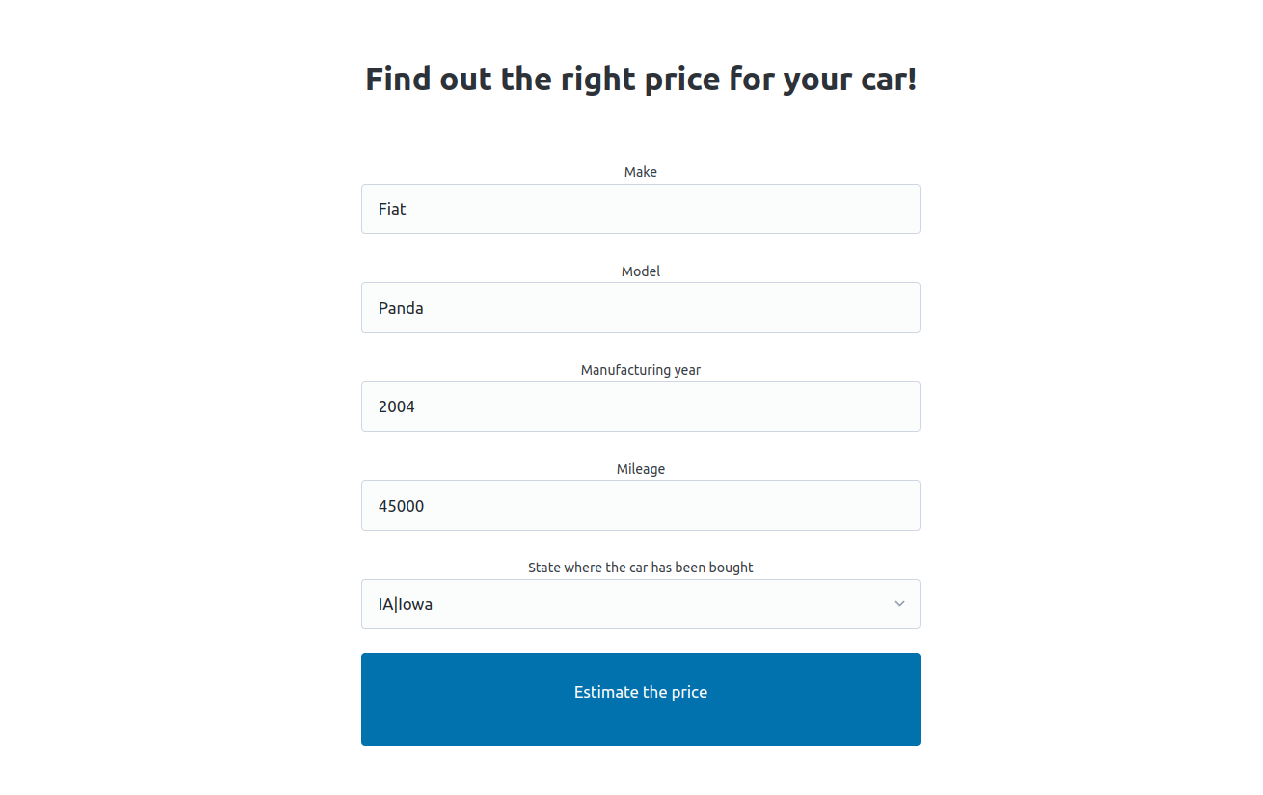
\includegraphics[width=12cm]{form}
        \centering
        \caption{Disponible sur la page d'accueil du site, ce formulaire permet à l'utilisateur d'entrer les caractéristiques de sa voiture pour obtenir une estimation}
        \centering
    \end{figure}
    \subsection{Les données disponibles}
    Pour nous permettre de mener notre mission à bien, l'Argus met à notre disposition un jeu de données qui recense plus de 800 000 ventes de voitures d'occasion. Pour chaque transaction sont indiqués :
    \begin{itemize}
        \item le prix de vente
        \item l'année de production de la voiture
        \item le nombre de kilomètres qu'elle a parcourus
        \item la ville où s'est déroulée la vente
        \item l'état américain où la vente a eu lieu
        \item le VIN, un identifiant unique pour chaque voiture
        \item la marque de la voiture
        \item son modèle.
    \end{itemize}
    \textbf{Remarque}: le jeu de données présenté ci-dessus est disponible \href{https://www.kaggle.com/datasets/harikrishnareddyb/used-car-price-predictions/data}{ici}.
    Par ailleurs, le client nous fait savoir qu'il reçoit chaque mois de nouvelles informations sur le même schéma, qu'il stocke dans une base de données. Ces données pourront être utilisées pour améliorer le modèle et vérifier qu'il reste performant.
    \subsection{Exigences du client}
    Le client a quelques exigences très spécifiques en ce qui concerne le service d'intelligence artificielle dont il a besoin. Celles-ci sont les suivantes :
    \begin{itemize}
        \item l'équipe informatique d'IArgus doit disposer d'un moyen qui leur permette de visualiser simplement les performances des l'intelligence artificielle, afin de s'apercevoir rapidement de tout problème
        \item Les estimations de prix d'IArgus doivent être suffisamment précises pour être exploitables par l'utilisateur. Ainsi, le seuil suivant nous est imposé : \textbf{l'intelligence artificielle doit produire des estimations de prix qui sont égales aux prix "réels" contenus dans les bases de données de l'Argus, avec une tolérance de +/- 20\%}. \item dans le cas où ce seuil de 20\% serait dépassé, l'équipe informatique veut immédiatement en être avertie par e-mail
        \item enfin, les dirigeants de l'Argus souhaite que l'accès au service d'IA soit sécurisé, afin que seuls l'application IArgus et les membres de l'équipe de développement puissent l'utiliser.
    \end{itemize}
    \section{Architecture du projet}
    Le service d'IA est constitué de plusieurs composants :
    \begin{itemize}
        \item un modèle d'intelligence artificielle entraîné avec les données fournies par l'Argus. Il prédit ensuite une estimation de prix en fonction des données entrées par l'utilisateur.
        \item une API qui expose ce modèle. C'est le seul composant qui interagit avec l'application web IArgus. Lorsque l'utilisateur soumet un formulaire avec les informations de son véhicule, celles-ci sont automatiquement transmises de façon sécurisée à l'API via une requête HTTP. L'API communique ensuite avec le modèle pour obtenir une estimation de prix et renvoie le résultat à l'application, qui peut l'afficher pour l'utilisateur. 
        \item un dashboard qui permet aux techniciens de l'équipe informatique de visualiser l'évaluation des performances du modèle et de voir l'historique des entraînements et tests réalisés
        \item un script de monitorage. Exécuté une fois par mois pour tenir compte des nouvelles données reçues, il teste le modèle avec les nouvelles données et lance un nouvel entraînement si ses performances se sont trop dégradées (i.e. si l'erreur moyenne du modèle a dépassé 20\%). Dans le cas où l'erreur resterait malgré tout trop élevée après cela, le script envoie une alerte par e-mail à l'équipe technique.
        \item une base de données qui stocke toutes les données utilisées par le modèle. Les nouvelles données reçues chaque mois par l'Argus y sont automatiquement ajoutées.
    \end{itemize}
    [Mettre un schéma général ici qui montre le modèle, l'API, le script de monitoring, le serveur MLflow et la BDD]

    \subsection{Le modèle d'intelligence artificielle}
    Le modèle d'intelligence artificielle utilisé pour réaliser les estimations de prix est un \textbf{Deep Neural Network} (abrégé DNN), ou \textbf{Réseau Neuronal Profond} en français. Un réseau neuronal est une type de modèle d'intelligence artificielle inspiré par le cerveau humain, plus précisément par les neurones et les connexions synaptiques entre eux. C'est un type de machine learning appelé deep learning qui consiste à utiliser des neurones ou nodes interconnectés, organisés en plusieurs couches. Ce modèle a été choisi suite à la réalisation d'un processus de benchmarking qui a opposé le DNN à plusieurs autres modèles tels que SGD et SVR.

    [Comparaison hors du cadre du dossier. Dans la version finale (après le rendu du premier avril), ajouter un résumé des modèles testés et résultats obtenus en annexe et y ajouter une référence.]
    
    [SCHÉMA DE LA STRUCTURE DU RÉSEAU]

    Toutes les données disponibles ne sont pas utilisées par le modèle. Parmi les données disponibles pour chaque vente de voiture [AJOUTER LIEN], seules les informations suivantes sont utilisées :
    \begin{itemize}
        \item le prix de vente
        \item l'année de production de la voiture
        \item le nombre de kilomètres qu'elle a parcourus
        \item l'état américain où la vente a eu lieu
        \item la marque de la voiture
        \item son modèle.
    \end{itemize}
    Le VIN n'est pas utilisé car il s'agit d'un identifiant purement administratif destiné à assurer le suivi d'un véhicule unique. Il est créé à partir d'informations tells que la ville de production de la voiture, un code de sécurité, et le numéro de série de la voiture, entre autres données. Les informations pertinentes incluses dans ce numéro telles que la marque de la voiture étant déjà disponibles dans notre jeu de données, nous n'utiliserons donc pas le VIN ici.
    La ville où se déroule la vente de voiture n'est pas non plus utilisée par notre modèle. Dans ce cas, ce choix est fait dans un souci de performances. En effet, un DNN ne peut traiter que des données numériques : les informations telles que la marque de la voiture, son modèle, la ville ou l'état de la transaction doivent être \textbf{encodées} pour être exploitables par le modèle d'IA. Ceci est accompli grâce à la technique du \textbf{One-Hot Encoding}, qui consiste à convertir des valeurs discrètes (telles qu'un nom de marque par exemple) en vecteurs constitués de 1 et de 0 uniquement. Or, la taille de ce vecteur dépend du nombre de valeurs uniques présentes dans nos données pour chaque variable (56 dans le cas de l'état, par exemple). Convertir la ville par cette technique génèrerait des vecteurs à plusieurs milliers de dimensions, ce qui augmenterait considérablement les besoins en terme de mémoire vive et de puissance de calcul. Toutes ces raisons expliquent pourquoi la ville de vente a été mise de côté.
    
    Une fois que notre DNN est entraîné avec les données fournies par l'Argus, il devient possible de l'utiliser pour estimer des prix de vente. Cependant, l'application n'interagit pas directement avec le modèle. À la place elle envoie des requêtes à un composant qui fait office d'intermédiaire, \textbf{l'API}.
    \subsection{l'API}
    L'accès au modèle est contrôlé par une API (\textbf{Application Programming Interface}). Une API sert de façade à un ensemble de fonctionnalités : elle permet à un tiers d'utiliser ces fonctionnalités sans avoir besoin de connaître leur fonctionnement interne. Dans notre cas, notre API permet à des tiers (l'application IArgus, les techniciens de l'équipe de développement) d'utiliser notre modèle d'IA sans connaître les rouages de son fonctionnement.

    Utiliser une API pour donner accès à un service confère plusieurs avantages :
    \begin{itemize}
        \item offrir une fonctionnalité via une API permet de contrôler qui accède à notre service, et de quelle manière. En ce qui concerne IArgus, des système d'authentification, de cryptage des communications et de validation des données fournies sont notamment mis en place
        \item les API web telles que celle utilisée dans ce projet permettent de standardiser les communications avec l'API. Dans la mesure où toutes les requêtes à l'API sont réalisées selon le protocole HTTP, il devient possible d'intégrer rapidement les fonctionnalités de l'API à d'autres projets en cas de besoin
        \item il existe plusieurs outils et frameworks qui permettent de mettre en place rapidement des API. 
    \end{itemize}
    Une API web accepte des requêtes via plusieurs \textbf{endpoints} ("points de terminaison" en français). Chaque endpoint peut accepter une ou plusieurs méthodes de requêtes HTTP. Voici les points de terminaison utilisés par l'API d'IArgus :
    \begin{itemize}
        \item / (racine de l'API) : ce endpoint renvoie un message d'aide qui explique comment utiliser l'API. Il accepte la méthode GET
        \item /predict : permet de demander à l'IA une estimation de prix à partir des informations envoyées avec la requête. Ce endpoint accepte les requêtes POST.
    \end{itemize}
    Afin de répondre aux exigences du client concernant la sécurisation de l'accès au modèle, plusieurs mécanismes de sécurité ont été implémentés pour réguler l'accès au modèle et protéger l'API des cyberattaques. Le premier de ces mécanismes est la création d'un mécanisme d'authentification via un token secret. Selon cette mécanique, les utilisateurs qui font une requête à l'API doivent y joindre une clé secrète transmise uniquement aux utilisateurs autorisés (pour plus de sécurité, cette clé est automatiquement renouvelée à intervalles réguliers). Les requêtes sans clé valide sont refusées par l'API, ce qui permet d'éviter que des utilisateurs extérieurs à l'entreprise ou des pirates informatiques n'utilisent l'API sans permission.

    Un autre mécanisme de sécurité implémenté est la limitation du nombre de requêtes qu'un utilisateur peut envoyer à l'API dans un court laps de temps. Cela nous permet de protéger notre système des attaques par déni de service, qui consistent à effectuer un grand nombre de requêtes à une URL en un temps très court afin de submerger les capacités du serveur et de le rendre hors service. Dans notre cas, cette protection est d'autant plus importante que notre modèle d'IA consomme beaucoup de mémoire et de ressources de calcul. Ainsi, un grand nombre de requêtes simultanées à /predict pourrait rapidement submerger le serveur où notre IA est déployée.

    Notre API utilise également le protocole \textbf{HTTPS} pour plus de sécurité. Cette extension du protocole HTTP permet de crypter les données qui circulent entre le serveur où se trouve l'API et les clients. Ainsi, il devient impossible pour un pirate informatique d'espionner les données qui circulent entre l'application IArgus et l'API (comme des clés d'API secrètes, par exemple).

    Enfin, notre API réalise une validation des données qu'elle reçoit. Autrement dit, des mécanismes ont été mis en place pour s'assurer que les informations envoyées par l'utilisateur sont bien conformes à ce qui est attendu. Pour le endpoint /predict, par exemple, cela consiste à s'assurer que le nom de l'état est bien une chaîne de caractères, l'année un entier, etc... Ceci nous permet de nous assurer qu'un utilisateur distrait ou mal intentionné ne peut pas faire bugger notre système en envoyant le mauvais type de données.

    L'API a été développée en Python avec le framework FastAPI. FastAPI permet de développer des API web rapidement, en minimisant les temps de calcul nécessaires pour l'API. De plus, FastAPI offre des fonctionnalités qui permettent de rapidement mettre en place des mécanismes tels que la limitation du nombre de requêtes ou la validation des données entrantes.
    \subsection{Suivi du modèle}

    Le suivi du modèle englobe les composants qui nous permettent de visualiser les performances du modèle au cours du temps et d'envoyer des alertes si jamais celles-ci passent en-dessous d'un seuil acceptable. 
    
    Avant de détailler le fonctionnement de ces composants, parlons de la métrique utilisée pour évaluer les performances de notre modèle. Lors de la présentation des exigences du client[INSÉRER LIEN], nous avons vu que ce dernier souhaitait garantir que les prix prédits se situaient en moyenne dans un intervalle de 20\% autour des prix réels. Ce critère de performances correspond à \textbf{l'erreur absolue moyenne en pourcentage}, souvent appelée \textbf{MAPE} pour "Mean Absolute Percentage Error". Cette métrique nous indique le pourcentage moyen d'erreur d'un modèle par rapport aux valeurs réelles, ce qui correspond bien à ce que nous demande notre client. Par conséquent, \textbf{la MAPE sera utilisée comme métrique de référence dans la suite de ce dossier.} On considèrera ainsi qu'une MAPE de 0.2 (soit 20\% d'erreur) resprésente le seuil de performances à ne pas dépasser. Un modèle qui a une MAPE supérieure à ce seuil devra donc être \textbf{réentraîné}.

    \begin{figure}[h!]
        \begin{equation}MAPE = \frac {\sum \frac{\lvert A-F \rvert}{A} \times 100}{N}  \end{equation}
        \centering
        \caption{Définition de la MAPE. Ici $N$ représente le nombre total de prédictions réalisées, $A$ est la valeur réelle du prix, et $F$ la valeur prédite par le modèle d'IA}
        \centering
    \end{figure}

    Le suivi du modèle est assuré par trois composants de notre projet :
    \begin{itemize}
        \item un dashboard généré par MLflow, hébergé sur un serveur local
        \item un script exécuté automatiquement à intervalles réguliers qui teste le modèle, le réentraîne si besoin et envoie des alertes par e-mail en cas de problème
        \item la base de données qui contient toutes les informations concernant les ventes de voitures d'occasion, continuellement alimentée par l'Argus.
    \end{itemize}

    [SCREENSHOT DE MLflow]

    [SCREENSHOT QUI MONTRE LE MAIL D'ALERTE REÇU]

    \subsection{Tests et intégration continue}
    \section{Intégration du service dans l'application}

    [PENSER À METTRE UN SCREENSHOT DU RÉSULTAT DE LA PRÉCISION TEL QU'AFFICHÉ DANS L'APPLICATION WEB]

    \section{Packaging et mise en place du modèle}

    \newpage
    \section*{Conclusion}
    

    \addcontentsline{toc}{section}{Conclusion}

    \newpage
    \begin{thebibliography}{5}
    \end{thebibliography}

    \end{document}